% Options for packages loaded elsewhere
\PassOptionsToPackage{unicode}{hyperref}
\PassOptionsToPackage{hyphens}{url}
%
\documentclass[
]{article}
\usepackage{amsmath,amssymb}
\usepackage{iftex}
\ifPDFTeX
  \usepackage[T1]{fontenc}
  \usepackage[utf8]{inputenc}
  \usepackage{textcomp} % provide euro and other symbols
\else % if luatex or xetex
  \usepackage{unicode-math} % this also loads fontspec
  \defaultfontfeatures{Scale=MatchLowercase}
  \defaultfontfeatures[\rmfamily]{Ligatures=TeX,Scale=1}
\fi
\usepackage{lmodern}
\ifPDFTeX\else
  % xetex/luatex font selection
\fi
% Use upquote if available, for straight quotes in verbatim environments
\IfFileExists{upquote.sty}{\usepackage{upquote}}{}
\IfFileExists{microtype.sty}{% use microtype if available
  \usepackage[]{microtype}
  \UseMicrotypeSet[protrusion]{basicmath} % disable protrusion for tt fonts
}{}
\makeatletter
\@ifundefined{KOMAClassName}{% if non-KOMA class
  \IfFileExists{parskip.sty}{%
    \usepackage{parskip}
  }{% else
    \setlength{\parindent}{0pt}
    \setlength{\parskip}{6pt plus 2pt minus 1pt}}
}{% if KOMA class
  \KOMAoptions{parskip=half}}
\makeatother
\usepackage{xcolor}
\usepackage[margin=1in]{geometry}
\usepackage{longtable,booktabs,array}
\usepackage{calc} % for calculating minipage widths
% Correct order of tables after \paragraph or \subparagraph
\usepackage{etoolbox}
\makeatletter
\patchcmd\longtable{\par}{\if@noskipsec\mbox{}\fi\par}{}{}
\makeatother
% Allow footnotes in longtable head/foot
\IfFileExists{footnotehyper.sty}{\usepackage{footnotehyper}}{\usepackage{footnote}}
\makesavenoteenv{longtable}
\usepackage{graphicx}
\makeatletter
\def\maxwidth{\ifdim\Gin@nat@width>\linewidth\linewidth\else\Gin@nat@width\fi}
\def\maxheight{\ifdim\Gin@nat@height>\textheight\textheight\else\Gin@nat@height\fi}
\makeatother
% Scale images if necessary, so that they will not overflow the page
% margins by default, and it is still possible to overwrite the defaults
% using explicit options in \includegraphics[width, height, ...]{}
\setkeys{Gin}{width=\maxwidth,height=\maxheight,keepaspectratio}
% Set default figure placement to htbp
\makeatletter
\def\fps@figure{htbp}
\makeatother
\setlength{\emergencystretch}{3em} % prevent overfull lines
\providecommand{\tightlist}{%
  \setlength{\itemsep}{0pt}\setlength{\parskip}{0pt}}
\setcounter{secnumdepth}{5}
\ifLuaTeX
  \usepackage{selnolig}  % disable illegal ligatures
\fi
\IfFileExists{bookmark.sty}{\usepackage{bookmark}}{\usepackage{hyperref}}
\IfFileExists{xurl.sty}{\usepackage{xurl}}{} % add URL line breaks if available
\urlstyle{same}
\hypersetup{
  pdftitle={Kleefstra Syndrome Disease Concept Model},
  pdfauthor={Teaching Fellow - Minh Thu Bui; Supervisor - Professor Masanao Yajima; Wuge Li, Maysen Pagan, Amie Thomas},
  hidelinks,
  pdfcreator={LaTeX via pandoc}}

\title{\textbf{Kleefstra Syndrome Disease Concept Model}}
\author{Teaching Fellow - Minh Thu Bui \and Supervisor - Professor Masanao Yajima \and Wuge Li, Maysen Pagan, Amie Thomas}
\date{}

\begin{document}
\maketitle

\hypertarget{project-background-and-objectives}{%
\section{Project Background and Objectives}\label{project-background-and-objectives}}

The objective of this project is to create an interpretable visualization of the results produced by Kristen Connors' Disease Concept Model on Kleefstra Syndrome. The visualization should show which symptoms and impacts were discussed the most during interviews with the healthcare providers and caregivers of children with the condition. The results should indicate which symptoms/impacts are the most significant for the specified age groups in the eyes of the caregiver. It should give insight in to how Kleefstra Syndrome impacts the lives of caregivers and those afflicted by the condition.

\hypertarget{visualizations}{%
\section{Visualizations}\label{visualizations}}

\hypertarget{total-frequencies-bar-plot}{%
\subsection{Total Frequencies Bar Plot}\label{total-frequencies-bar-plot}}

The most effective method for displaying the total number of references is by using a bar chart. This visual representation includes four distinct categories: ``KS Defining Concepts'', ``KS Individual Impact'', ``Caregiver Impact'', and ``Age''. Each depicted with varying colors to differentiate between them. Additionally, the data is organized in descending order to enable a clearer comparison of the references in each different categories.

\begin{figure}
\centering
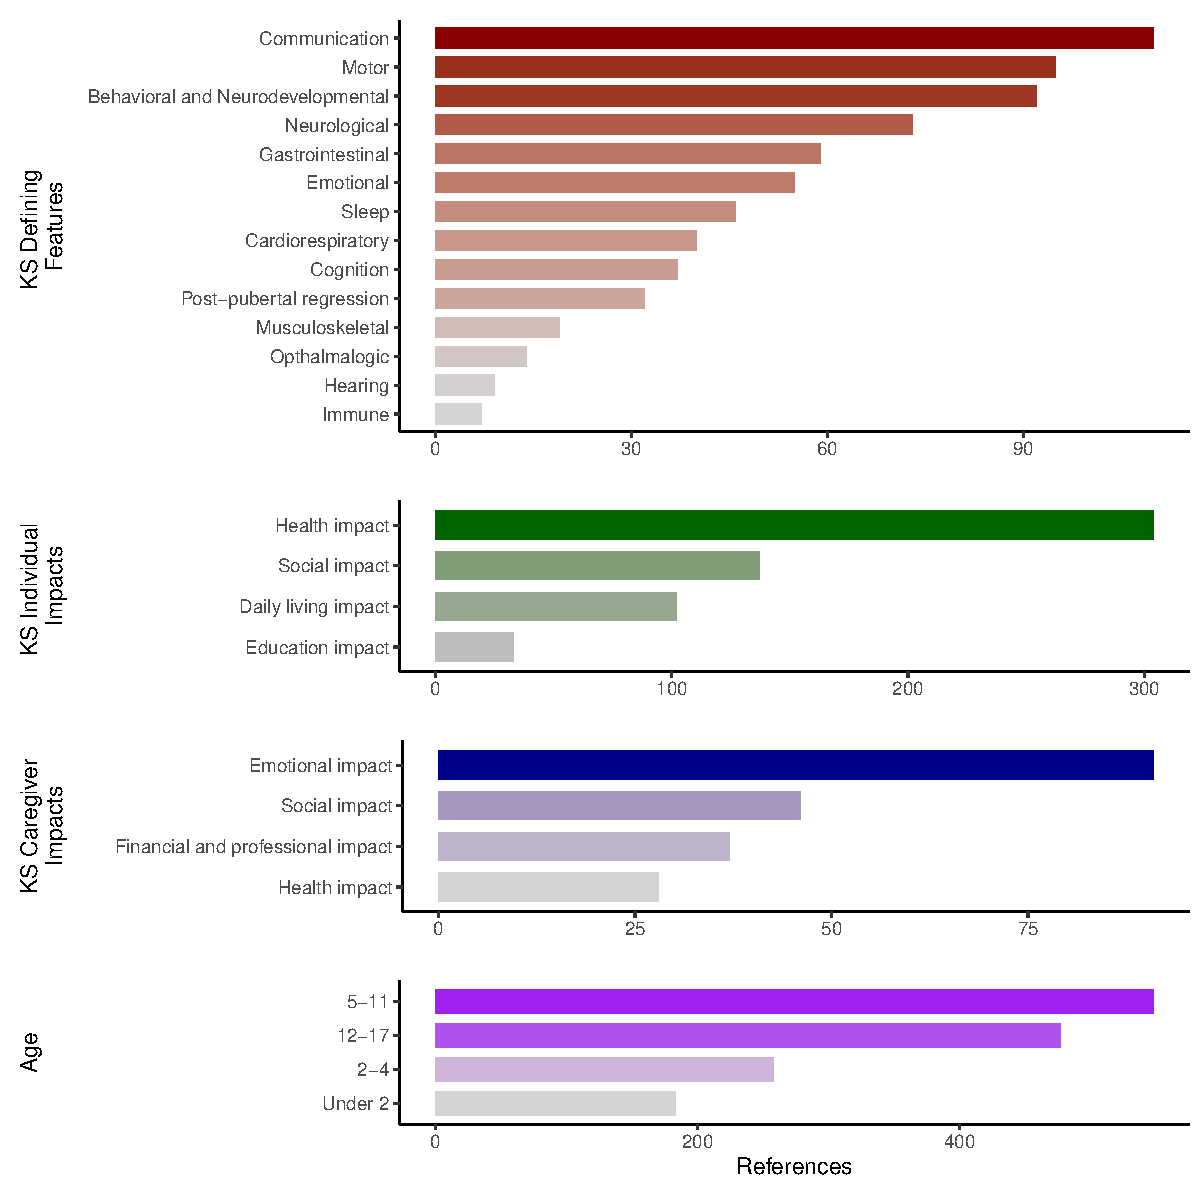
\includegraphics{Report_files/figure-latex/bar-plot-1.pdf}
\caption{\label{fig:bar-plot}Total references bar chart.}
\end{figure}

\hypertarget{analysis}{%
\subsubsection{Analysis}\label{analysis}}

\hypertarget{age-group-symptoms-frequencies-heatmap}{%
\subsection{Age Group Symptoms Frequencies Heatmap}\label{age-group-symptoms-frequencies-heatmap}}

Heatmaps are a great way to reveal relationships between variables. By representing numerical values with colors, heatmaps make it easier to identify areas of high and low values. For Figure \ref{fig:freq-plot} the frequency of each symptom was calculated by finding the sum of all symptoms mentioned per age group then dividing by the number that the specific symptom was mentioned. This normalizes the data so that the different response sizes are no longer an issue, making the age groups comparable.

\begin{verbatim}
## Warning: 程辑包'ggpubr'是用R版本4.3.2 来建造的
\end{verbatim}

\begin{verbatim}
## Warning: 程辑包'readr'是用R版本4.3.2 来建造的
\end{verbatim}

\begin{verbatim}
## Warning: 程辑包'stringr'是用R版本4.3.2 来建造的
\end{verbatim}

\begin{verbatim}
## Warning: 程辑包'lubridate'是用R版本4.3.2 来建造的
\end{verbatim}

\begin{figure}
\centering
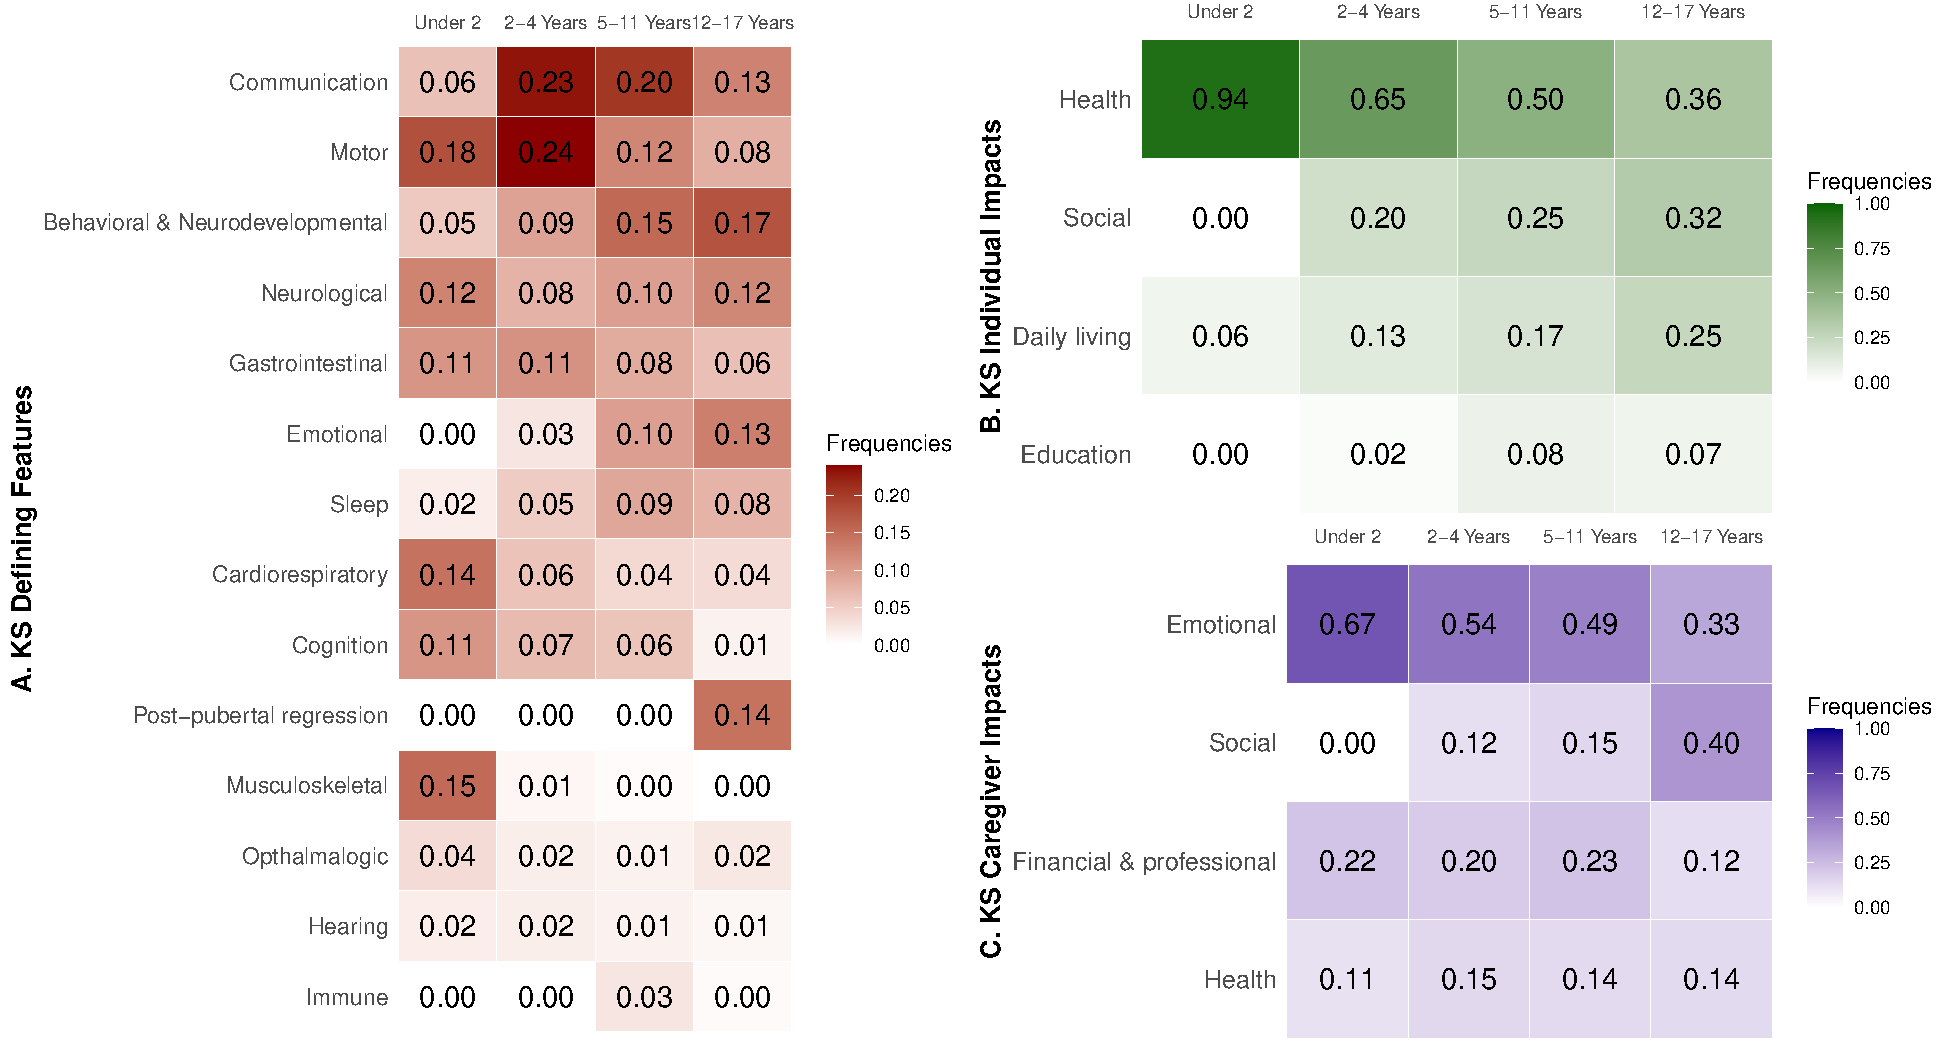
\includegraphics{Report_files/figure-latex/freq-plot-1.pdf}
\caption{\label{fig:freq-plot}Heatmap of references frequencies.}
\end{figure}

\hypertarget{analysis-1}{%
\subsubsection{Analysis}\label{analysis-1}}

Interpreting the graph can be done like the following. For the ``Impacts on Caregiver'' heatmap (bottom right graph) we can see that the emotional impacts were mentioned at a higher frequency than all other impacts for the Under 2 category. Emotional impact continues to be the most talked about for ages 2-4 and 5-11. Then comes second place to social impacts for age category 12-17.

The ``Symptoms'' heatmap is an a scale from 0.00-0.25, whereas the ``Impacts on Caregiver'' and ``Impacts on Individual'' are on a 0.00-1.00 scale. The reasoning is that the symptom most mentioned in interviews had a frequency of 0.24. Putting the heatmap on a 0.00-1.00 scale made it less visually effective for comparison purposes.

\hypertarget{age-group-frequencies-bar-plot}{%
\subsection{Age Group Frequencies Bar Plot}\label{age-group-frequencies-bar-plot}}

Another visualization that allows you to observe changes in the frequencies of references over different age groups is a stacked bar plot. Figure \ref{fig:stacked-plot} shows stacked bar plots for the frequencies of referenced KS Defining Concepts, KS Individual Concepts, and KS Caregiver Impacts. The different colors in each plot represent different concepts or impacts and the labeled frequencies represent the most referenced concept or impact for that age group.

\begin{figure}
\centering
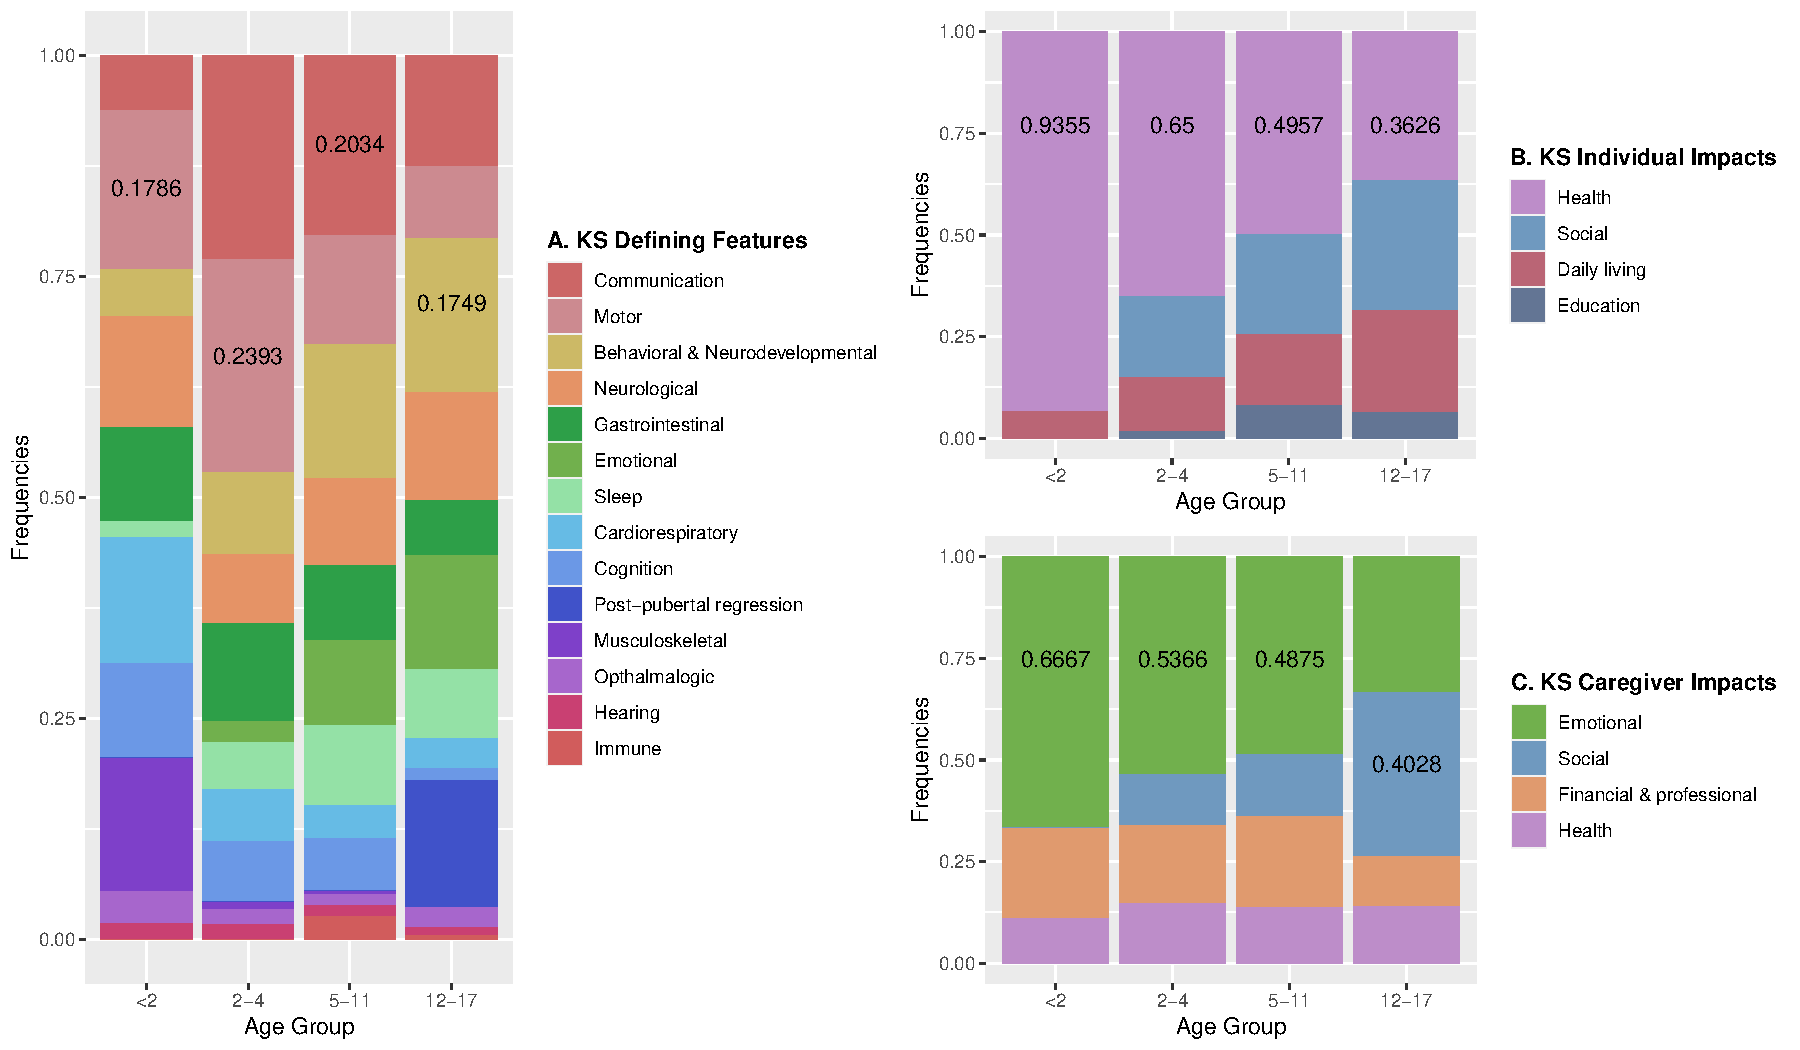
\includegraphics{Report_files/figure-latex/stacked-plot-1.pdf}
\caption{\label{fig:stacked-plot}Stacked bar plot of references frequencies. Labeled frequencies represent the most frequent concept or impact for that age group.}
\end{figure}

\hypertarget{analysis-2}{%
\subsubsection{Analysis}\label{analysis-2}}

These stacked bar plots are a great way to observe changes in the frequency of references across different age groups at a high level. For example, in stacked bar plot B, it is clear to see that health is the most referenced individual impact for children under the age of 2. However, as the age groups increase, the references to health decreases. This suggests that the significance of the child's health decreases as the child gets older when other impacts like social and daily living impacts begin to matter more. A similar pattern can be seen in bar plot C. As the age groups increase in age, the frequencies of references to emotional caregiver impacts decreases while social impacts increase.

There is a challenge with the interpretability of stacked bar plots. While the patterns mentioned above are clear to see looking at the plots, there is a difficulty in comparing concepts or impacts when they do not start at a common baseline. For example in bar plot A, it is hard to compare the references to gastrointestinal concepts between the age groups of less than 2 and 2 to 4 year olds. Additionally, due to the stacked nature of the bar plots, it is also difficult to determine what the exact frequency is of the referenced concept or impact unless it is the bottom bar.

\hypertarget{conclusion}{%
\subsubsection{Conclusion}\label{conclusion}}

\end{document}
